%\section{Weitere Spiele}
%M�gen die Spiele beginnen

\begin{appendix}
\chapter{Messergebnisse}
\label{app}
\begin{table}[thb]
\caption{Location Versuch 1}
\begin{tabular}{l|l|l|}
\cline{2-3}
                                      & locationClient         & locationManager         \\ \hline
\multicolumn{1}{|l|}{Datum}           & \multicolumn{2}{l|}{10.12.2014}                  \\ \hline
\multicolumn{1}{|l|}{Ort}             & \multicolumn{2}{l|}{Universit�t Koblenz, Campus} \\ \hline
\multicolumn{1}{|l|}{Wetter}          & \multicolumn{2}{l|}{bew�lkt, leichter Niesel}     \\ \hline
\multicolumn{1}{|l|}{Ger�t}           & \multicolumn{2}{l|}{Samsung Galaxy S3}           \\ \hline
\multicolumn{1}{|l|}{Genauigkeit}     & 7,049                  & 8,698                   \\ \hline
\multicolumn{1}{|l|}{Updates/Sekunde} & 0,936                  & 1,016                   \\ \hline
\multicolumn{3}{l}{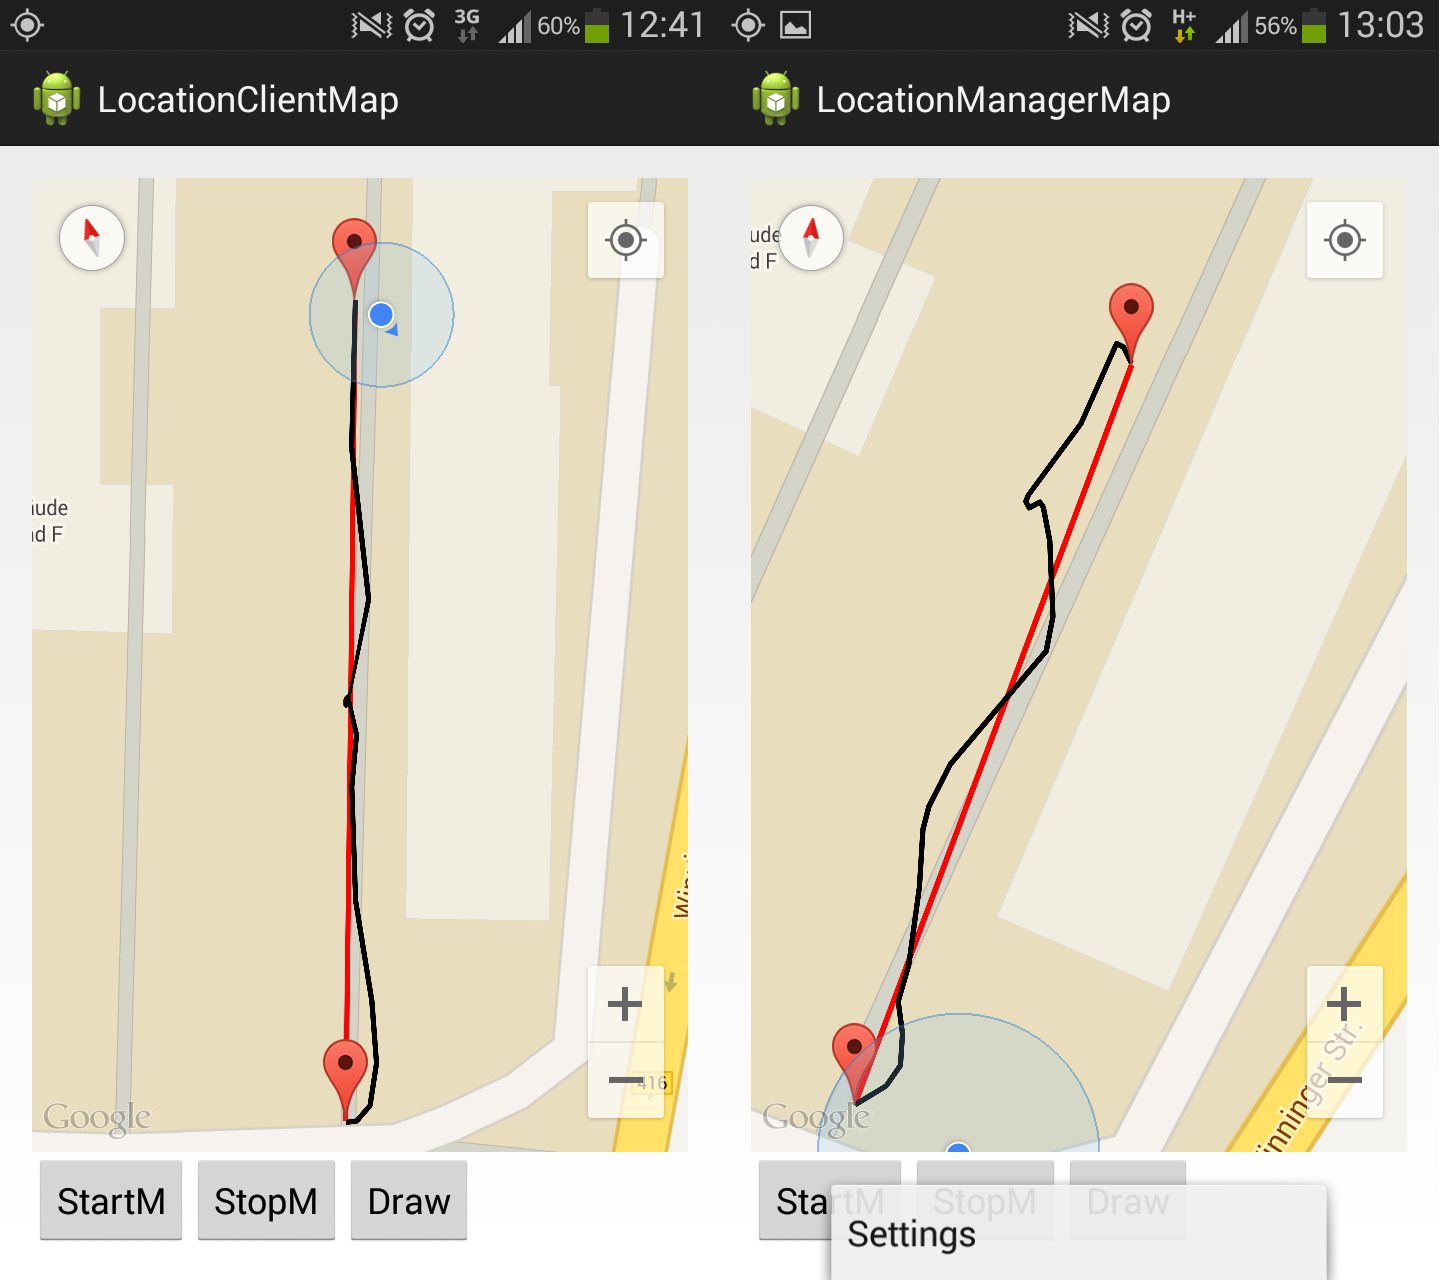
\includegraphics[width=0.5\textwidth]{4-Technische_Loesungen/4-1-Positionsermittlung/Data/Screenshot_2014-12-10-12-41-12_fuusion.png}}
\end{tabular}
\label{tab:lV1}
\end{table}


\begin{table}[thb]
\caption{Location Versuch 2}
\begin{tabular}{l|l|l|}
\cline{2-3}
                                      & locationClient                & locationManager                \\ \hline
\multicolumn{1}{|l|}{Datum}           & \multicolumn{2}{l|}{14.12.2014}                                \\ \hline
\multicolumn{1}{|l|}{Ort}             & \multicolumn{2}{l|}{Ransbach-Baumbach, L307 Richtung Mogendorf} \\ \hline
\multicolumn{1}{|l|}{Wetter}          & \multicolumn{2}{l|}{leicht bew�lkt leicht windig}       \\ \hline
\multicolumn{1}{|l|}{Ger�t}           & \multicolumn{2}{l|}{Samsung Galaxy S3}                         \\ \hline
\multicolumn{1}{|l|}{Genauigkeit}     & 5,482                         & 6,216                          \\ \hline
\multicolumn{1}{|l|}{Updates/Sekunde} & 1,003                         & 0,969                          \\ \hline
\multicolumn{3}{l}{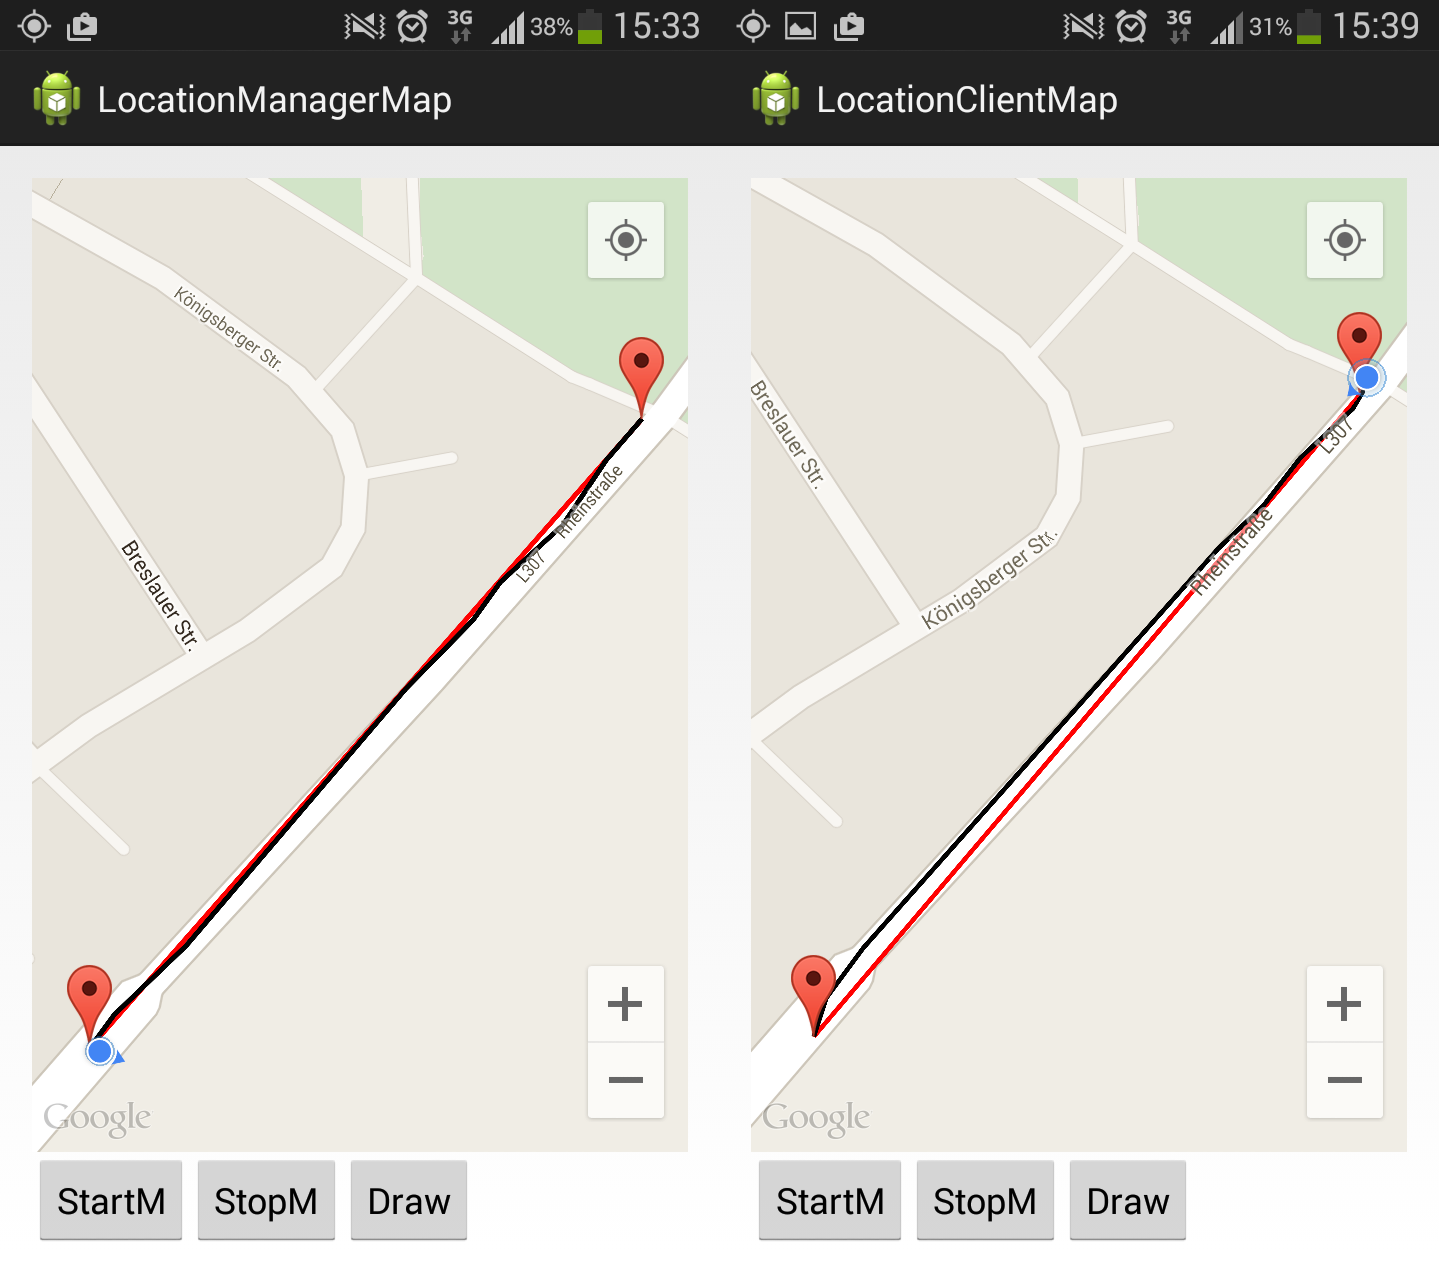
\includegraphics[width=0.5\textwidth]{4-Technische_Loesungen/4-1-Positionsermittlung/Data/Screenshot_2014-12-14-15-33-10_fuusion.png}}
\end{tabular}
\label{tab:lV2}
\end{table}

\begin{table}[thb]
\caption{Location Versuch 3}
\begin{tabular}{l|l|l|}
\cline{2-3}
                                      & locationClient                & locationManager                \\ \hline
\multicolumn{1}{|l|}{Datum}           & \multicolumn{2}{l|}{08.05.2015}                                \\ \hline
\multicolumn{1}{|l|}{Ort}             & \multicolumn{2}{l|}{Ransbach-Baumbach, L307 Richtung Mogendorf} \\ \hline
\multicolumn{1}{|l|}{Wetter}          & \multicolumn{2}{l|}{sonnig}       \\ \hline
\multicolumn{1}{|l|}{Ger�t}           & \multicolumn{2}{l|}{Samsung Galaxy S3}                         \\ \hline
\multicolumn{1}{|l|}{Genauigkeit}     & 5,616													& 5,303                          \\ \hline
\multicolumn{1}{|l|}{Updates/Sekunde} & 1,042                         & 1,004                          \\ \hline
\multicolumn{3}{l}{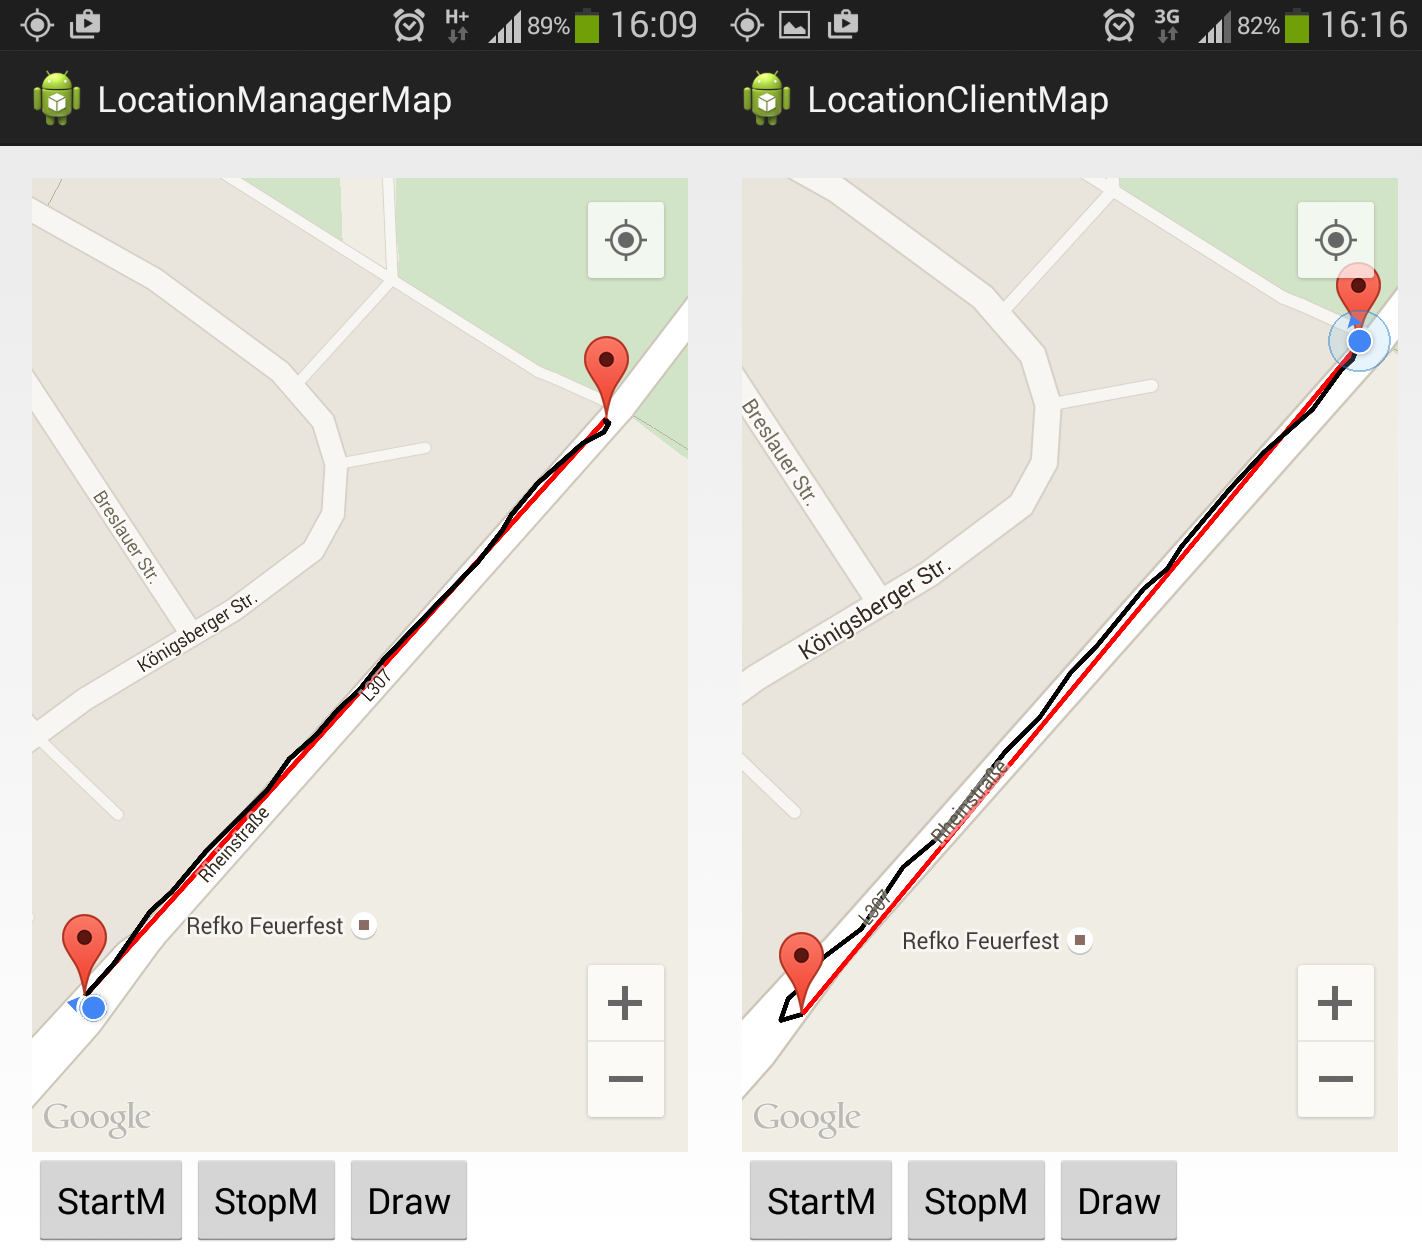
\includegraphics[width=0.5\textwidth]{4-Technische_Loesungen/4-1-Positionsermittlung/Data/Screenshot_2015-05-08-16-09-35_fuusion.png}}
\end{tabular}
\label{tab:lV3}
\end{table}


\begin{table}[thb]
\caption{Location Versuch 4}
\begin{tabular}{l|l|l|}
\cline{2-3}
                                      & locationClient                & locationManager                \\ \hline
\multicolumn{1}{|l|}{Datum}           & \multicolumn{2}{l|}{08.05.2015}                                \\ \hline
\multicolumn{1}{|l|}{Ort}             & \multicolumn{2}{l|}{Ransbach-Baumbach, L307richtung Mogendorf} \\ \hline
\multicolumn{1}{|l|}{Wetter}          & \multicolumn{2}{l|}{sonnig}       \\ \hline
\multicolumn{1}{|l|}{Ger�t}           & \multicolumn{2}{l|}{Samsung Galaxy S3}                         \\ \hline
\multicolumn{1}{|l|}{Genauigkeit}     & 6,163													& 5,868                          \\ \hline
\multicolumn{1}{|l|}{Updates/Sekunde} & 1,010													& 1,011 \\ \hline
\multicolumn{3}{l}{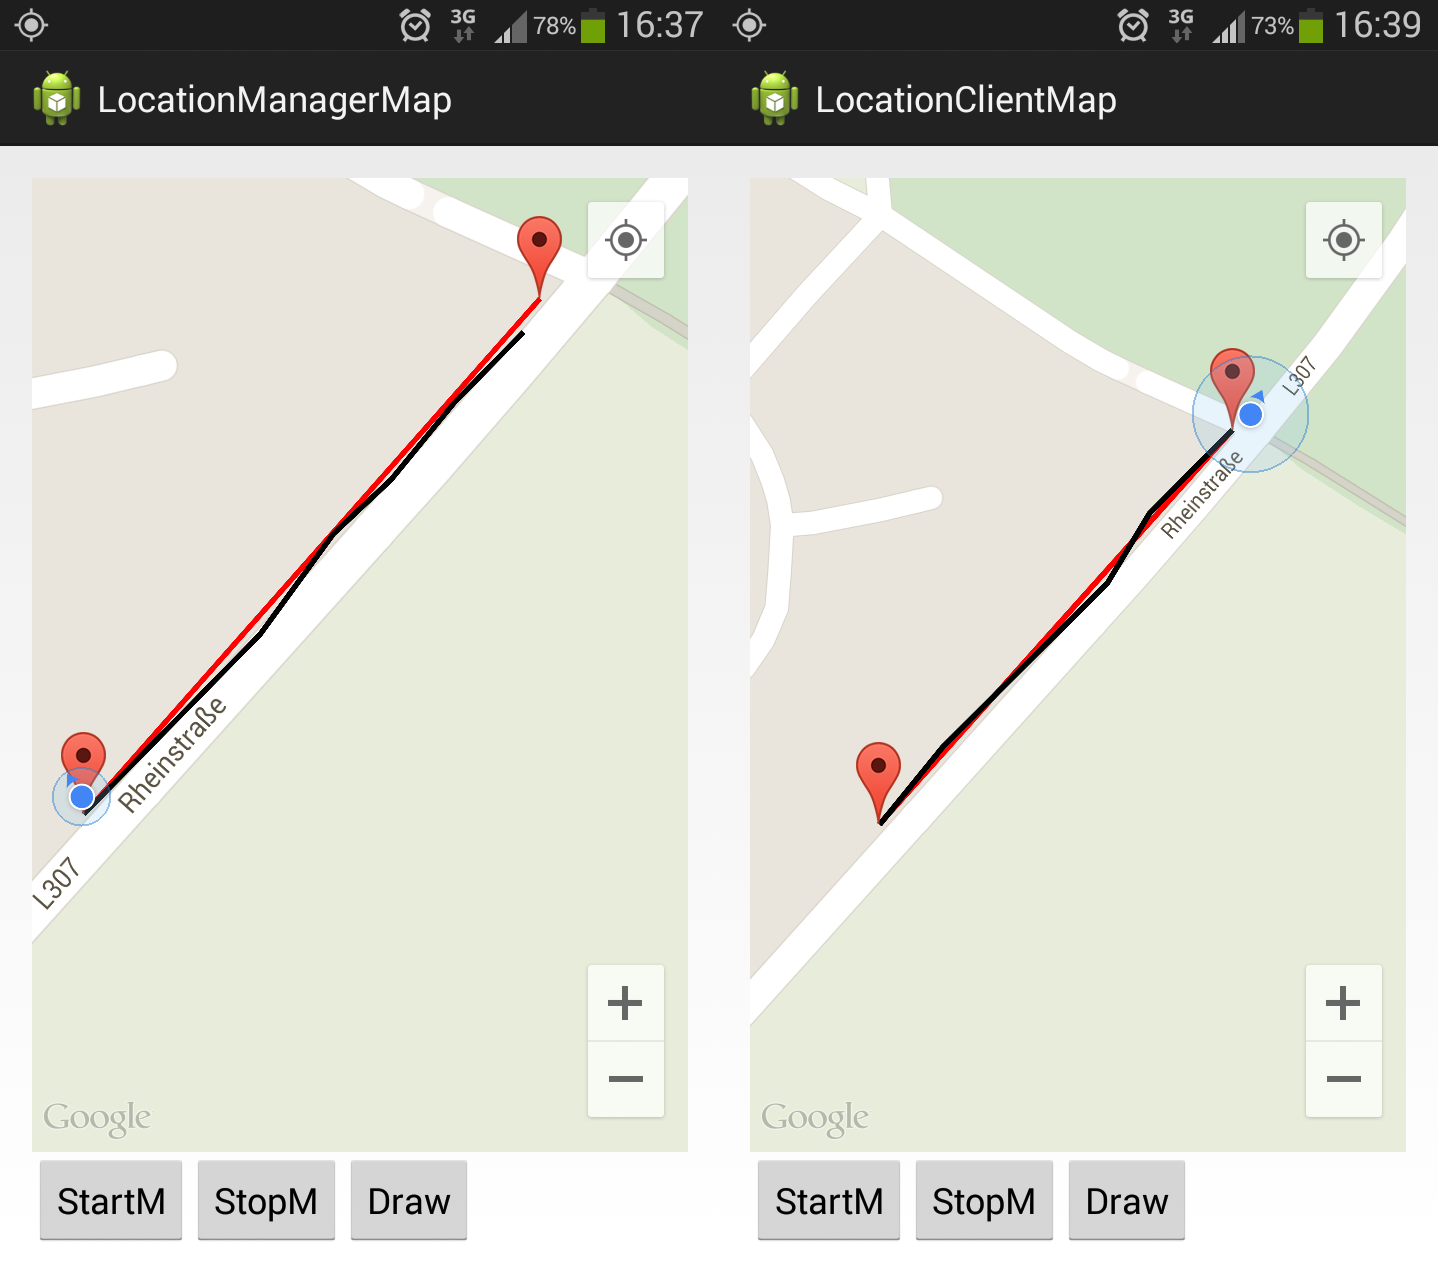
\includegraphics[width=0.5\textwidth]{4-Technische_Loesungen/4-1-Positionsermittlung/Data/Screenshot_2015-05-08-16-37-21_fuusion.png}}
\end{tabular}
\label{tab:lV4}
\end{table}


\begin{table}[thb]
\caption{Location Versuch 5}
\begin{tabular}{l|l|l|}
\cline{2-3}
                                      & locationClient                & locationManager                \\ \hline
\multicolumn{1}{|l|}{Datum}           & \multicolumn{2}{l|}{08.05.2015}                                \\ \hline
\multicolumn{1}{|l|}{Ort}             & \multicolumn{2}{l|}{Ransbach-Baumbach, L307richtung Mogendorf} \\ \hline
\multicolumn{1}{|l|}{Wetter}          & \multicolumn{2}{l|}{sonnig}       \\ \hline
\multicolumn{1}{|l|}{Ger�t}           & \multicolumn{2}{l|}{Samsung Galaxy S3}                         \\ \hline
\multicolumn{1}{|l|}{Genauigkeit}     & 5,473													& 6,317                          \\ \hline
\multicolumn{1}{|l|}{Updates/Sekunde} & 1,009													& 1 \\ \hline
\multicolumn{3}{l}{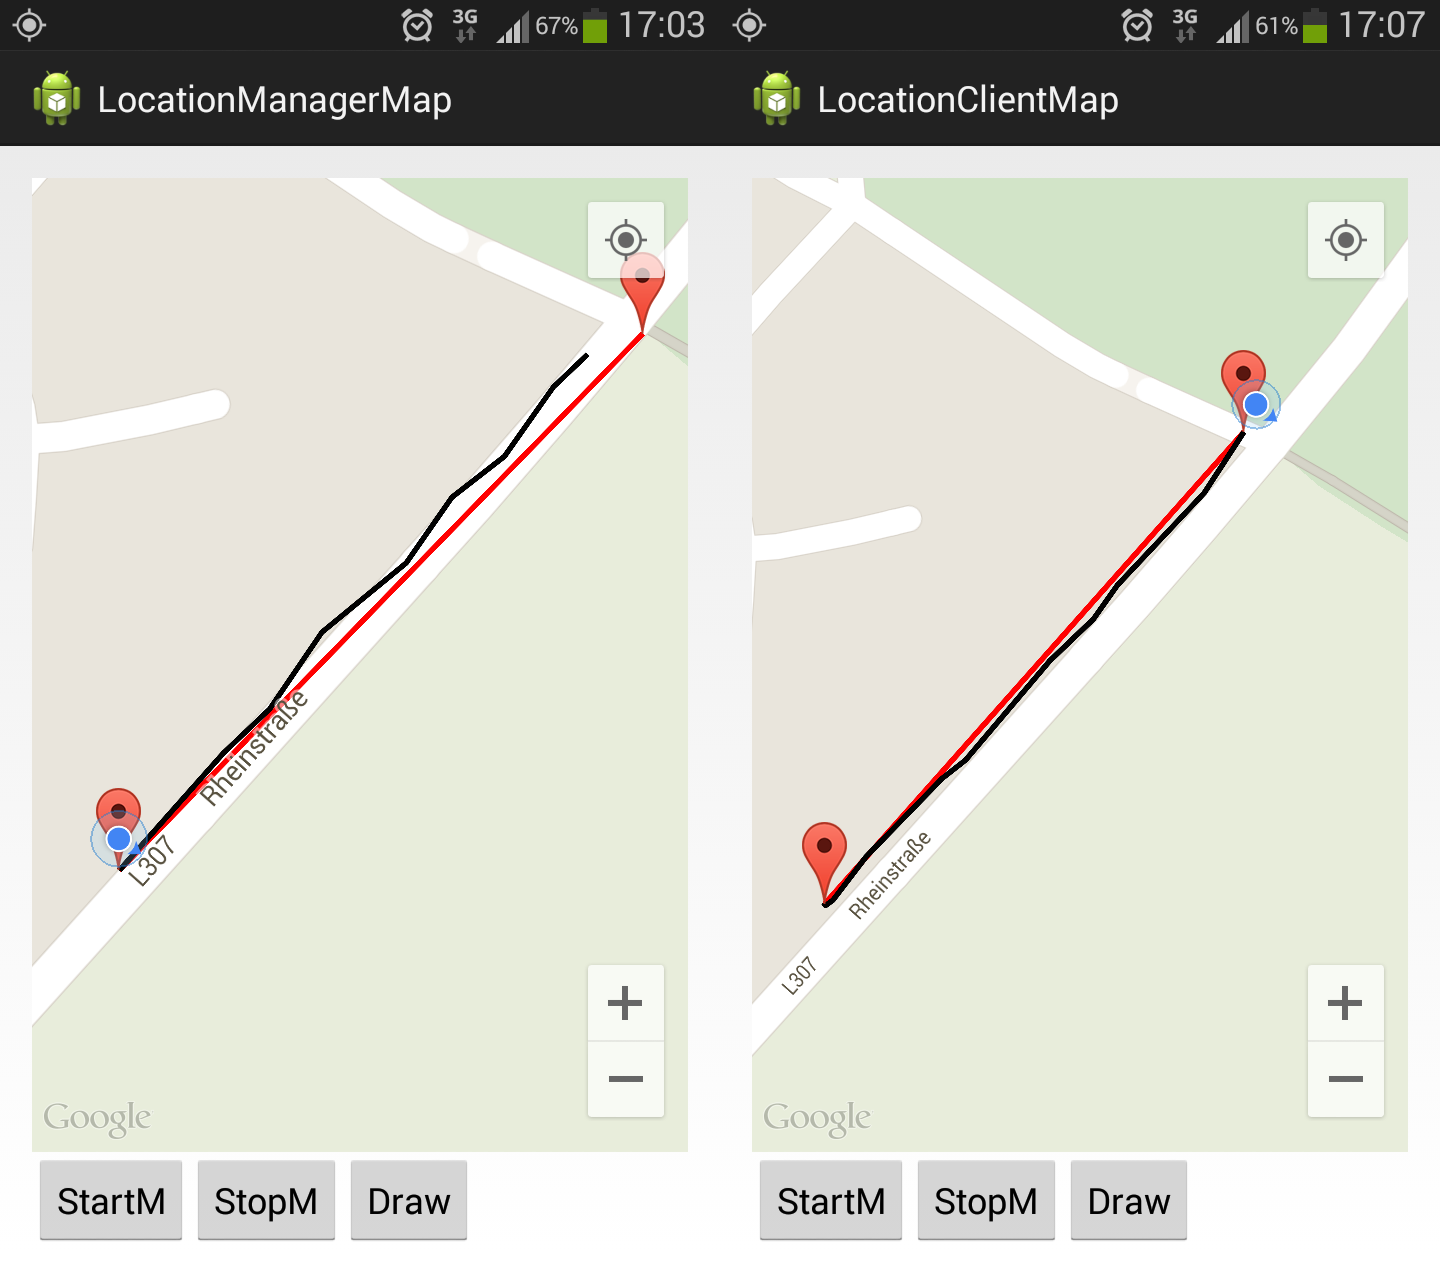
\includegraphics[width=0.5\textwidth]{4-Technische_Loesungen/4-1-Positionsermittlung/Data/Screenshot_2015-05-08-17-03-10_fuusion.png}}
\end{tabular}
\label{tab:lV5}
\end{table}

  
\begin{table}[thb]
\caption{Location Versuch 6}
\begin{tabular}{l|l|l|}
\cline{2-3}
                                      & locationClient                & locationManager                \\ \hline
\multicolumn{1}{|l|}{Datum}           & \multicolumn{2}{l|}{08.05.2015}                                \\ \hline
\multicolumn{1}{|l|}{Ort}             & \multicolumn{2}{l|}{Ransbach-Baumbach, L307richtung Mogendorf} \\ \hline
\multicolumn{1}{|l|}{Wetter}          & \multicolumn{2}{l|}{sonnig}       \\ \hline
\multicolumn{1}{|l|}{Ger�t}           & \multicolumn{2}{l|}{htc one s}                         \\ \hline
\multicolumn{1}{|l|}{Genauigkeit}     & 5,483													& 3,293                          \\ \hline
\multicolumn{1}{|l|}{Updates/Sekunde} & 1,047													& 0,967   \\ \hline
\multicolumn{3}{l}{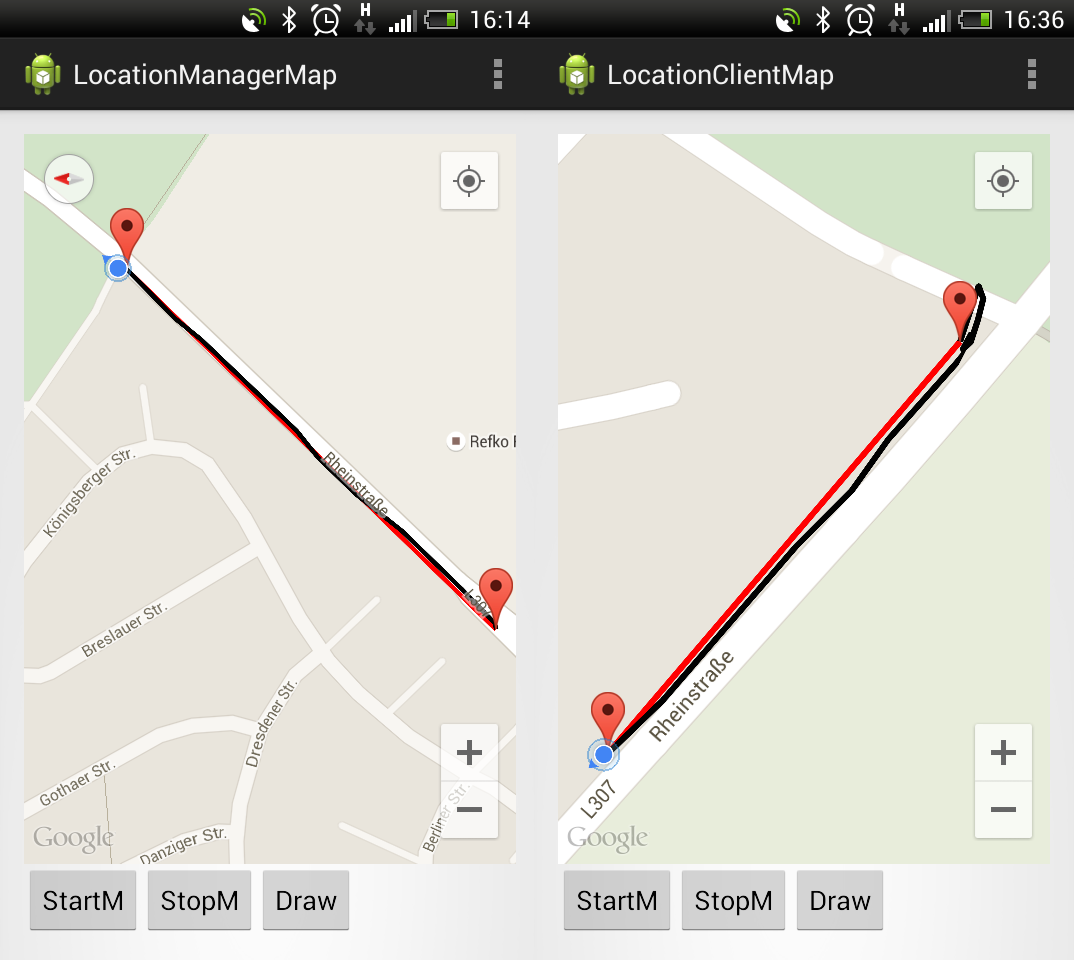
\includegraphics[width=0.5\textwidth]{4-Technische_Loesungen/4-1-Positionsermittlung/Data/2015-05-08_16-14-46_fuusion.png}}
\end{tabular}
\label{tab:lV6}
\end{table}


\begin{table}[thb]
\caption{Location Versuch 7}
\begin{tabular}{l|l|l|}
\cline{2-3}
                                      & locationClient                & locationManager                \\ \hline
\multicolumn{1}{|l|}{Datum}           & \multicolumn{2}{l|}{08.05.2015}                                \\ \hline
\multicolumn{1}{|l|}{Ort}             & \multicolumn{2}{l|}{Ransbach-Baumbach, L307richtung Mogendorf} \\ \hline
\multicolumn{1}{|l|}{Wetter}          & \multicolumn{2}{l|}{sonnig}       \\ \hline
\multicolumn{1}{|l|}{Ger�t}           & \multicolumn{2}{l|}{htc one s}                         \\ \hline
\multicolumn{1}{|l|}{Genauigkeit}     & 3,962													& 3,144                          \\ \hline
\multicolumn{1}{|l|}{Updates/Sekunde} & 1,070													& 1,009    \\ \hline
\multicolumn{3}{l}{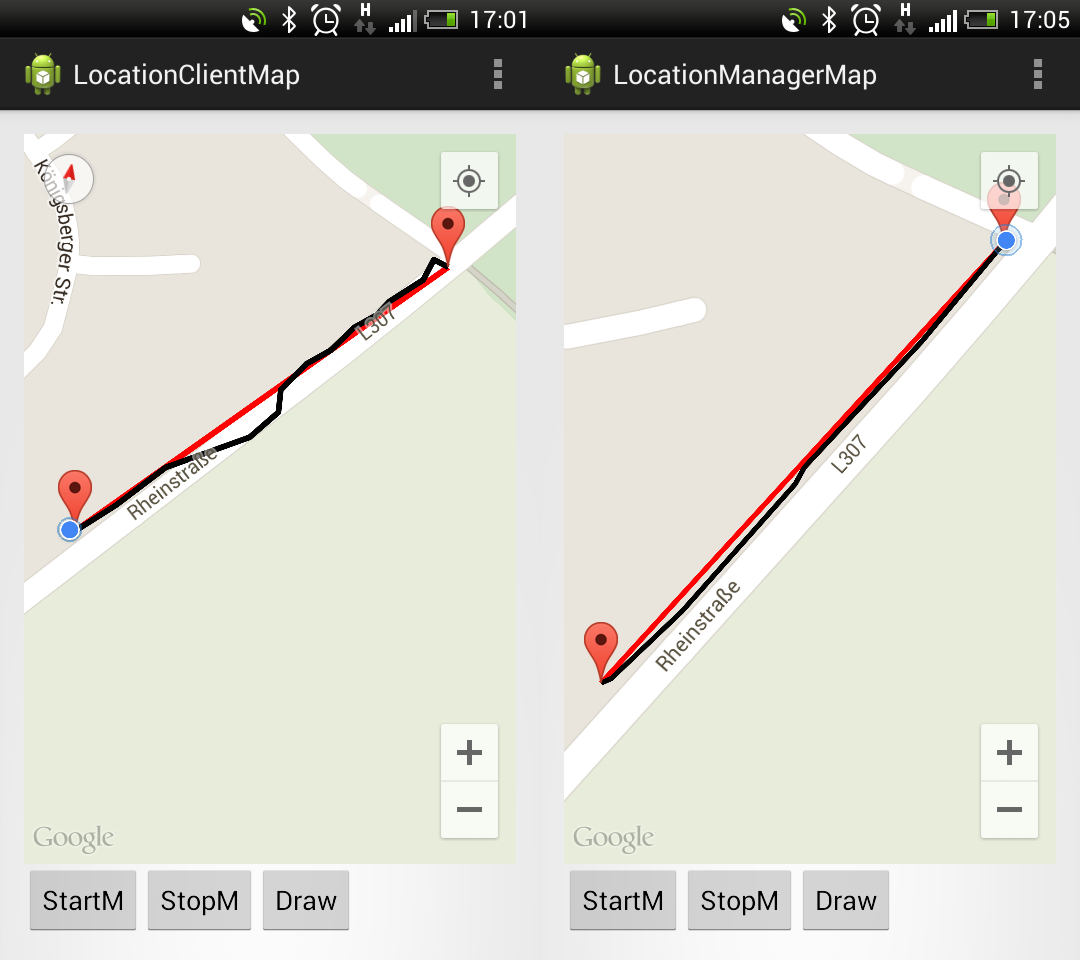
\includegraphics[width=0.5\textwidth]{4-Technische_Loesungen/4-1-Positionsermittlung/Data/2015-05-08_17-01-38_fuusion.png}}
\end{tabular}
\label{tab:lV7}
\end{table}



\begin{table}[thb]
\caption{Location Versuch 8}
\begin{tabular}{l|l|l|}
\cline{2-3}
                                      & locationClient                & locationManager                \\ \hline
\multicolumn{1}{|l|}{Datum}           & \multicolumn{2}{l|}{08.05.2015}                                \\ \hline
\multicolumn{1}{|l|}{Ort}             & \multicolumn{2}{l|}{Ransbach-Baumbach, L307richtung Mogendorf} \\ \hline
\multicolumn{1}{|l|}{Wetter}          & \multicolumn{2}{l|}{sonnig}       \\ \hline
\multicolumn{1}{|l|}{Ger�t}           & \multicolumn{2}{l|}{htc desire x}                         \\ \hline
\multicolumn{1}{|l|}{Genauigkeit}     & 12,722													& 7,576                          \\ \hline
\multicolumn{1}{|l|}{Updates/Sekunde} & 1,009 													& 1,008    \\ \hline
\multicolumn{3}{l}{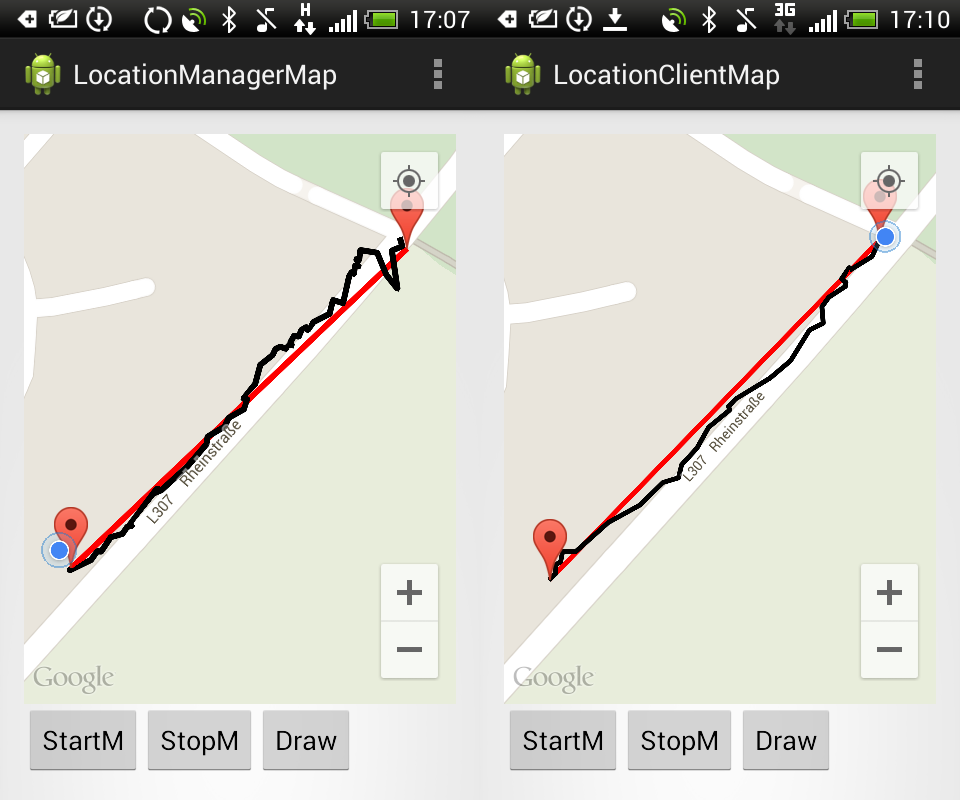
\includegraphics[width=0.5\textwidth]{4-Technische_Loesungen/4-1-Positionsermittlung/Data/Screenshot_2015-05-08-17-07-04_fuusion.png}}
\end{tabular}
\label{tab:lV8}
\end{table}


\begin{table}[thb]
\caption{Location Versuch 9}
\begin{tabular}{l|l|l|}
\cline{2-3}
                                      & locationClient                & locationManager                \\ \hline
\multicolumn{1}{|l|}{Datum}           & \multicolumn{2}{l|}{08.05.2015}                                \\ \hline
\multicolumn{1}{|l|}{Ort}             & \multicolumn{2}{l|}{Ransbach-Baumbach, L307richtung Mogendorf} \\ \hline
\multicolumn{1}{|l|}{Wetter}          & \multicolumn{2}{l|}{sonnig}       \\ \hline
\multicolumn{1}{|l|}{Ger�t}           & \multicolumn{2}{l|}{htc desire x}                         \\ \hline
\multicolumn{1}{|l|}{Genauigkeit}     & 6,436													& 5,281                    \\ \hline
\multicolumn{1}{|l|}{Updates/Sekunde} & 1,004 												& 0,981    \\ \hline
\multicolumn{3}{l}{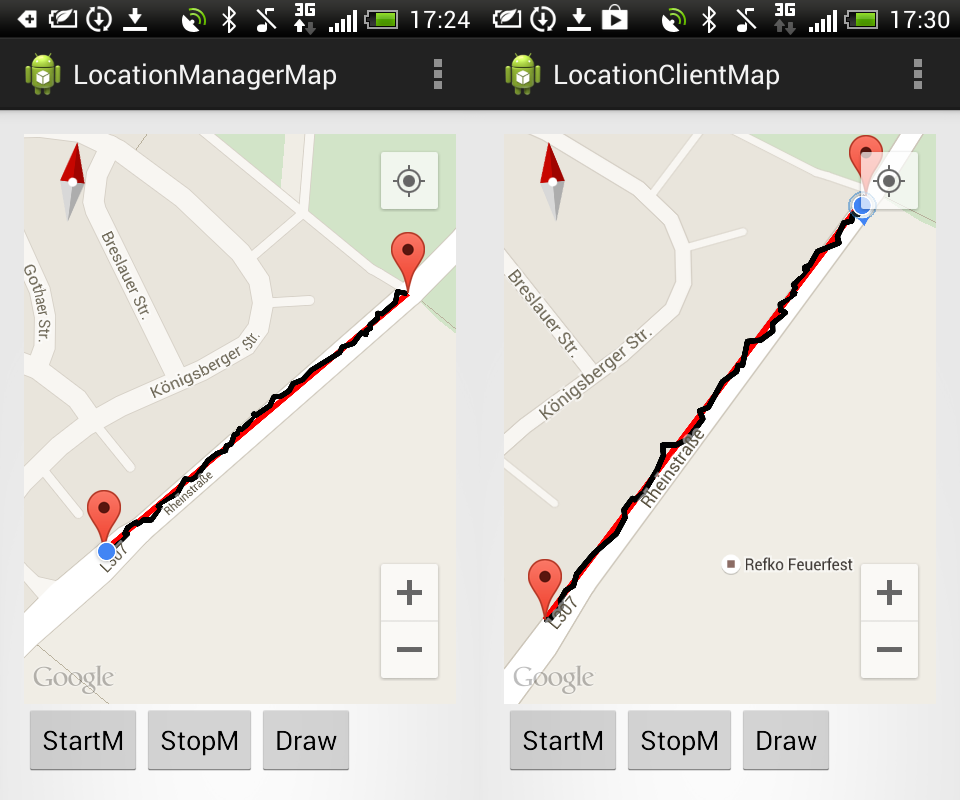
\includegraphics[width=0.5\textwidth]{4-Technische_Loesungen/4-1-Positionsermittlung/Data/Screenshot_2015-05-08-17-24-35_fuusion.png}}
\end{tabular}
\label{tab:lV9}
\end{table}


\begin{table}[thb]
\caption{Location Versuch 10}
\begin{tabular}{l|l|l|}
\cline{2-3}
                                      & locationClient                & locationManager                \\ \hline
\multicolumn{1}{|l|}{Datum}           & \multicolumn{2}{l|}{08.05.2015}                                \\ \hline
\multicolumn{1}{|l|}{Ort}             & \multicolumn{2}{l|}{Ransbach-Baumbach, L307richtung Mogendorf} \\ \hline
\multicolumn{1}{|l|}{Wetter}          & \multicolumn{2}{l|}{sonnig}       \\ \hline
\multicolumn{1}{|l|}{Ger�t}           & \multicolumn{2}{l|}{htc desire x}                         \\ \hline
\multicolumn{1}{|l|}{Genauigkeit}     & 7,848													& 5,500                    \\ \hline
\multicolumn{1}{|l|}{Updates/Sekunde} & 1,009 												& 0,952    \\ \hline
\multicolumn{3}{l}{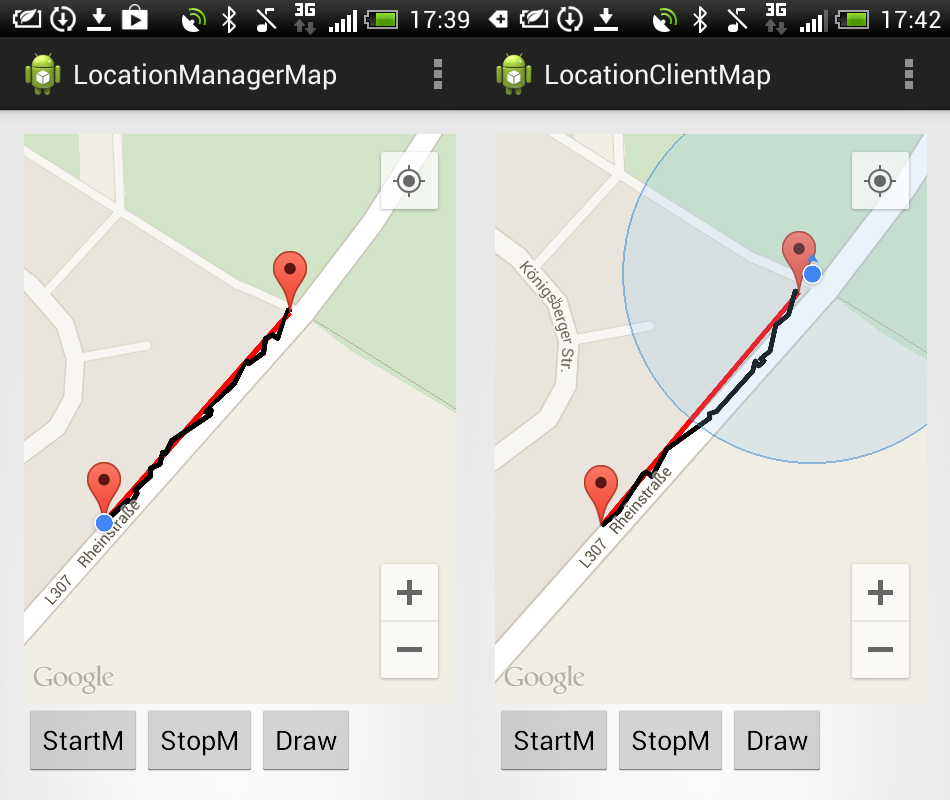
\includegraphics[width=0.5\textwidth]{4-Technische_Loesungen/4-1-Positionsermittlung/Data/Screenshot_2015-05-08-17-39-18_fuusion.png}}
\end{tabular}
\label{tab:lV10}
\end{table}

  
\begin{table}[thb]
\caption{Location Versuch 11}
\begin{tabular}{l|l|l|}
\cline{2-3}
                                      & locationClient                & locationManager                \\ \hline
\multicolumn{1}{|l|}{Datum}           & \multicolumn{2}{l|}{08.05.2015}                                \\ \hline
\multicolumn{1}{|l|}{Ort}             & \multicolumn{2}{l|}{Ransbach-Baumbach, L307richtung Mogendorf} \\ \hline
\multicolumn{1}{|l|}{Wetter}          & \multicolumn{2}{l|}{sonnig}       \\ \hline
\multicolumn{1}{|l|}{Ger�t}           & \multicolumn{2}{l|}{htc one s}                         \\ \hline
\multicolumn{1}{|l|}{Genauigkeit}     & 3,957													& 5,505                          \\ \hline
\multicolumn{1}{|l|}{Updates/Sekunde} & 1,107													& 1,018    \\ \hline
\multicolumn{3}{l}{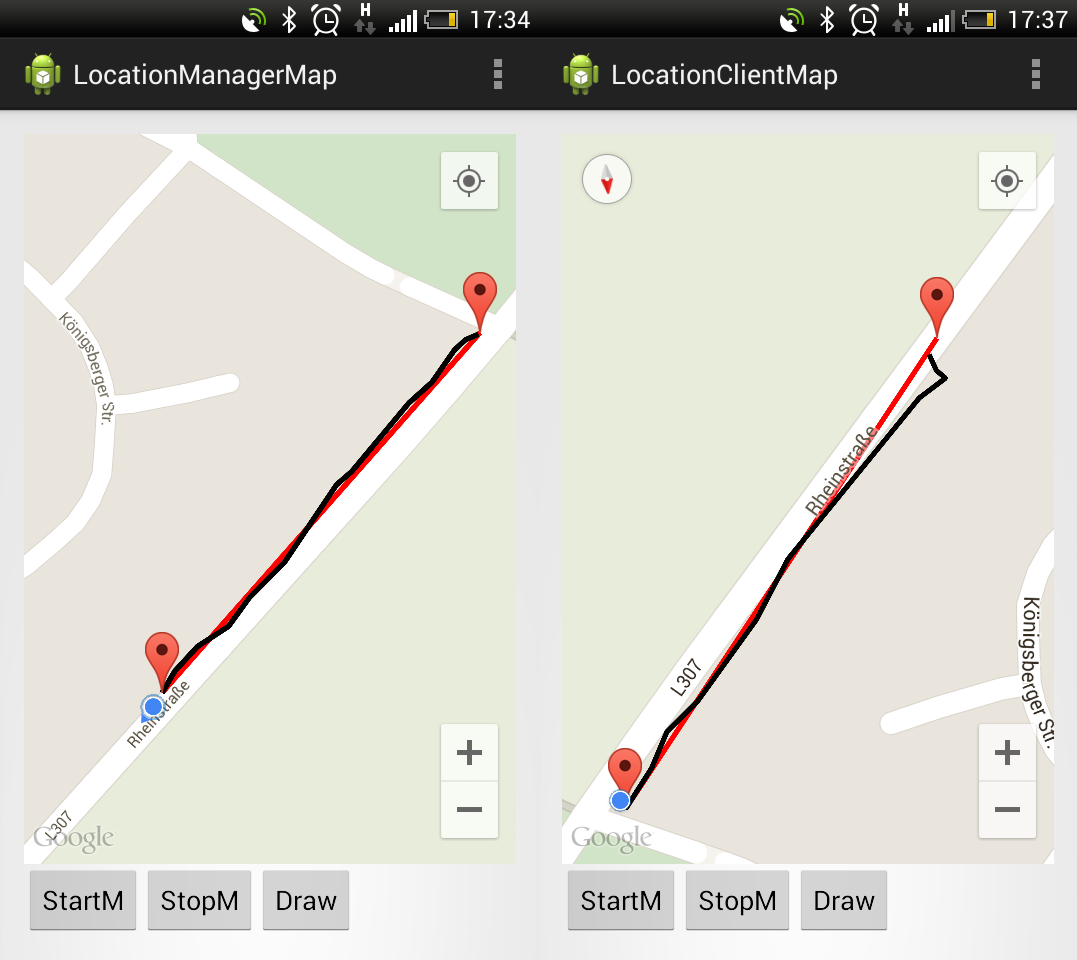
\includegraphics[width=0.5\textwidth]{4-Technische_Loesungen/4-1-Positionsermittlung/Data/2015-05-08_17-34-52_fuusion.png}}
\end{tabular}
\label{tab:lV11}
\end{table}
\end{appendix}